\documentclass[11pt, letterpaper, onecolumn]{article}

% Imports
\usepackage[english]{babel}
\usepackage{fancyhdr}
\usepackage{extramarks}
\usepackage{amsmath, amsthm, amsfonts,mathtools, framed, wasysym}
\usepackage[shortcuts]{extdash} % Use \-/ for hyphenated words
\usepackage{environ}
\usepackage{fancyvrb}
\usepackage[top=1.00in, bottom=1.00in, left=0.75in, right=0.75in]{geometry}
\usepackage{algorithm}
\usepackage{algpseudocode}
\usepackage{accents}
% Pseudocode enabler
\usepackage{listings}
\usepackage{color}

\definecolor{dkgreen}{rgb}{0,0.6,0}
\definecolor{gray}{rgb}{0.5,0.5,0.5}
\definecolor{mauve}{rgb}{0.58,0,0.82}

\lstset{frame=tb,
  language=Java,
  aboveskip=3mm,
  belowskip=3mm,
  showstringspaces=false,
  columns=flexible,
  basicstyle={\small\ttfamily},
  numbers=none,
  numberstyle=\tiny\color{gray},
  keywordstyle=\color{blue},
  commentstyle=\color{dkgreen},
  stringstyle=\color{mauve},
  breaklines=true,
  breakatwhitespace=true,
  tabsize=3
}

% tikz
\usepackage{pgf}
\usepackage{tikz}
\usetikzlibrary{arrows,automata}

% Page
\headsep=0.3in
\linespread{1.15}
\setlength\parindent{0pt}

% Horizontal Rules
\newcommand{\hwRuleWidth}{0.4pt}
\renewcommand\headrulewidth{\hwRuleWidth}
\renewcommand\footrulewidth{\hwRuleWidth}

% Header and Footer
\pagestyle{fancy}
\lhead{\hwAuthor\ (\hwSection)}
\chead{\hwClass\ (\hwInstructor): \hwTitle}
\rhead{\firstxmark}
\lfoot{\lastxmark}
\cfoot{\thepage}
\newcommand{\enterProblemHeader}[2]{
  \nobreak\extramarks{}{Problem \arabic{#1}.\arabic{#2} continued on next page\ldots}\nobreak{}
  \nobreak\extramarks{Problem \arabic{#1}.\arabic{#2} (continued)}{Problem \arabic{#1}.\arabic{#2} continued on next page\ldots}\nobreak{}
}
\newcommand{\exitProblemHeader}[2]{
  \nobreak\extramarks{Problem \arabic{#1}.\arabic{#2} (continued)}{Problem \arabic{#1}.\arabic{#2} continued on next page\ldots}\nobreak{}
  \nobreak\extramarks{Problem \arabic{#1}.\arabic{#2}}{}\nobreak{}
}

% Counters
\setcounter{secnumdepth}{0}
\newcounter{partCounter}
\setcounter{partCounter}{1}
\newcounter{hwProblemCounter}
\newcounter{hwSubProblemCounter}
\numberwithin{equation}{hwProblemCounter}
\numberwithin{figure}{hwProblemCounter}

% Environments
\newenvironment{problem}[3] {
  \setcounter{hwProblemCounter}{#2}
  \setcounter{hwSubProblemCounter}{#3}
  \setcounter{partCounter}{1}
  \enterProblemHeader{hwProblemCounter}{hwSubProblemCounter}

  \large{\textbf{Problem #2.#3: #1}}\\
}{
  \exitProblemHeader{hwProblemCounter}{hwSubProblemCounter}
}

\newcommand{\question}[2]{\textbf{(#1)\ }\ #2\\}

\newenvironment{Proof}[1][Proof]
  {\proof[#1]\leftskip=1cm\rightskip=1cm}
  {\endproof}
%-------------------------------------------------------------------------------
% Assignmnet Variables
%-------------------------------------------------------------------------------
\newcommand{\hwTitle}{Homework 1}
\newcommand{\hwDueDate}{Jan 26, 2017}
\newcommand{\hwClass}{CS 181}
\newcommand{\hwInstructor}{Amit Sahai}
\newcommand{\hwAuthor}{}
\newcommand{\hwSection}{804501476}
% First Problem
\setcounter{hwProblemCounter}{1}
\setcounter{hwSubProblemCounter}{0}

%-------------------------------------------------------------------------------
\begin{document}
%-------------------------------------------------------------------------------
% TITLE
%-------------------------------------------------------------------------------
{\centering
  \Large{\textbf{\hwTitle}}\\
  \vspace{0.1in}\normalsize{\hwDueDate}\\
  \vspace{0.1in}\textbf{\hwAuthor} (\hwSection)\\
  \vspace{0.1in}\rule{\textwidth}{\hwRuleWidth}}\\


%-------------------------------------------------------------------------------
% Problem 1.0
%------------------------------------------------------------------------------
\begin{problem}{}{1}{0}
  \begin{proof}
    Let $A$ and $B$ be regular then this implies that $\exists$ DFAs \\
    $M_1 = (Q_1, \Sigma_1, \delta_1, q_0, F)$ \\
    $M_2= (Q_2, \Sigma_2, \delta_2, q^{'}_0, F^{'})$ \\
    which recognize $A$ and $B$ respectively. \\
    We construct PDA $N = (Q, \Sigma, \delta ,q_{start}, F, \Gamma)$: \\
    1) $Q = q_{start} \cup Q_1 \cup Q_2$ \\
    2) $\Sigma = \Sigma_1 \cup \Sigma_2$ \\
    3) $\Gamma = \{\$, u \in \Sigma_1\}$ \\
    4) $\delta^{'}(r \in Q, a \in \Sigma, b) =
    \begin{cases}
      \{q_0, (\varepsilon, \varepsilon \to \$ )\}, \ \text{if $r = q_{start}$} \\
      \{\delta_1(r, a), (a, \varepsilon  \to a) \}, \ \text{if $a \in \Sigma_1$} \\
      \{q^{'}_0,  (a, b \to \varepsilon) \}, \text{if $r \in F$, $a \in \Sigma_2$ and $b \in \Sigma_1$} \\
      \{\delta_2(r, a), (a, b \to \varepsilon) \}, \ \text{if $a \in \Sigma_2$ and $b \in \Sigma_1$} \\
      \{ q_{end}, (\varepsilon, \$ \to \varepsilon) \}, \ \text{if $r \in F^{'}$}
    \end{cases}$ \\
    5) $q_{start}$ \\
    6) $F^{''} = q_{end}$ \\ \\
    \textbf{Claim}: $N$ accepts $A \nabla B \iff M_1 \ \text{accepts}
    \ A \ \text{and} \ M_2 \ \text{accepts} \ B$ \\
    ($\Leftarrow$)
    Let $x \in A$ and $y \in B$ s.t $|x|=|y|=n$. Now $M_1$ recognizes $x$
    as follows: $\exists$ states $a_1,a_2,\dots,a_n$ s.t
    $\delta_1(a_i, x_i)= \{a_j \in Q_1\}$, $a_1 = q_0$, and $a_n \in F$.
    $M_2$ recognizes y as follows: $\exists$ states $b_1,b_2,\dots,b_n$ s.t
    $\delta_2(b_i, y_i) = \{b_j \in Q_2\}$, $b_1 = q^{'}_0$, and $b_n \in F$.
    Now the states $a_1,a_2,\dots,a_n,b_1,b_2,\dots,b_n$ is a concatenation
    of paths from $M_1$ to $M_2$ machine N has start state $q_{start}$ which
    makes an epsilon transition to $q_0 = a_1$ and will only get to $q_{end}$ if
    it has gone through $q^{'}_0 \in F^{'}$. This machine begins with an empty stack
    and pushes every character from x into the stack and will only accept if y has an equal amount of
    chararacters since $|x|=|y|=n$ we accept.\\
    ($\Rightarrow$)
    Let $z = z_1z_2 \dots z_{2n} \in A \nabla B$. Now machine N recognizes
    z as follows $\exists$ states $r_0r_1r_2 \dots r_{2n+1}$ and strings
    $s_0s_1\dots s_{n+1} \in \Gamma^{*}$ s.t $\delta(r_i, s_i, a) = (r_{i+1}, b)$
    s.t $s_i = at$ and $s_{i+1} = bt$ for $a,b \in \Gamma$ and $t \in \Gamma^{*}$.
    We also have that $r_0 = q_{start}$, $s_0 = \$ $, $r_{2n+1} = q_{end}$. Now the
    states $r_0r_1r_2 \dots r_{2n+1}$ correspond to the states
    $q_{new}, a_1,a_2, \dots, a_n, b_1, b_2, \dots, b_n, q_{end}$. The states
    $a_1, a_2, \dots, a_n$ are a computational path on machine $M_1$ and the
    states $b_1, b_2, \dots, b_n$ are a computational path on machine $M_2$.
    \\
    We have proved equivalency between PDA's and CFG $\implies A\nabla B$ is a CFL. 
   \end{proof}
\end{problem}

\newpage
%-------------------------------------------------------------------------------
% Problem 2.0
%-------------------------------------------------------------------------------
\begin{problem}{}{2}{0} \\
  \textbf{a.} \\
  $L$ regular $\implies \exists$ DFA $M=(Q,\Sigma, \delta, q_o,F)$. \\
  We construct $G_L = (V, \Sigma, R, S)$: \\
  1) $V=Q$ \\
  2) $\Sigma = \Sigma$ \\
  3) $S = q_0$ \\
  4) $R =
  \begin{cases}
    q^{'} \to a q^{''}, \ \ \text{if} \ \delta(q^{'},a)=q^{''} \\
    q^{'} \to \varepsilon, \ \ \text{if} \ \delta(q^{'}, a) = q^{''} \ and \ q^{''} \in F
  \end{cases}$ \\
  
  \textbf{Claim: $G_L$ generates L}
  \begin{proof} $ $ \\
    ($\Rightarrow$) By construction of $G_L$ every $w \in G_L$ creates a
    computation path on $M \implies w \in L$ \\
    ($\Leftarrow$) $\forall \ w=w_1w_2\dots W_n \in L$ then $\exists$ a computation path
    on $M$, $q_0q_1q_2 \dots q_{n+1}$. By construction of $G_L$, in deriving w,
    the start symbol of w's derivation is $q_0$ and we continue to derive
    using $\delta$ to pick the next variable as such
    \begin{align}
      q_0 \to w_1q_1 \to w_1w_2q_2 \to \dots \to w_nq_{n+1} 
    \end{align}
    The set of variables produces is the same computational path on M, so
    $w$ is generated by $G_L$.
  \end{proof}
  
  \textbf{b.}
  $G=(V,\Sigma, R, S)$ be a regular grammar this implies for every variable
  $A \in V$ we have the following set of rules. \\
  1) $A \to aB$ \\
  2) $A \to a$ \\
  3) $A \to \varepsilon$ \\
  where $a$ is a terminal symbol and $B$, $a \in \Sigma$ ad $B \in V$. \\
  We construct NFA $N = (Q, \Sigma, \delta, q_0, F)$ as follows: \\
  1) $Q = \{q_{i} \ | \ q_i \in V\}$ \\
  2) $\Sigma = \Sigma$ \\
  3) $q_0 = S$ \\
  4) $F = q_{end}$ \\
  5) $\delta(q_i, a \in \Sigma) = 
  \begin{cases}
    \delta(q_i, a) = q_j,  \ \text{if} \ q_i \to aq_j \\
    q_{end},  \ \text{if} \ q_i \to \varepsilon \ | \ a
  \end{cases} $
  \begin{proof}
    ($\Rightarrow$)
    By construction of $N$ every $w \in L$ which N accepts is a valid derivation
    from a regular grammar $G$. \\
    ($\Leftarrow$)
    $\forall w=w_1w_2 \dots w_n \in G \ \exists$ a derivation
    \begin{align}
      S \to w_1V_1 \to w_2V_2 \to \dots \to w_n V_n  
    \end{align}
    By construction of N $S=q_o$ and the variables $V_i$ correspond to states in
    N s.t. $\delta(V_j, a) = V_i$ so w induces a computational path on M and
    a terminal rule such as $v_i \to a \ | \ \varepsilon$ is a transitiion onto
    an accepting state of N. Therefore $w$ is accepted $\implies$ $w \in L$.
  \end{proof}
\end{problem}
%-------------------------------------------------------------------------------
% Problem 3.0
%-------------------------------------------------------------------------------
\begin{problem}{}{3}{0}
\textbf{a)} 
For $x$ and $y$ to be different they have to be different in at least one place.
\begin{align}
  \{0 \cup 1\}^a x_i \{0 \cup 1\}^b \$ \{0 \cup 1\}^a y_i \{0 \cup 1\}^c
\end{align}  
We construct a non-deterministic PDA M that reads $x$ and pushes $\blacksmiley{}$ onto the stack as a counter for the index before position $i$. We non-determinitically guess where $i$
is and what symbol $x_i$ is and push it onto the stack. We continue to read $x$ without performing any action until we reach $\$$. We transition according the the top of the stack, $x_i$, and pop. As we read $y$ we pop the $\blacksmiley{}$, this will index to position $y_i$ and if they are different then there is transition if not the machine dies. 
 

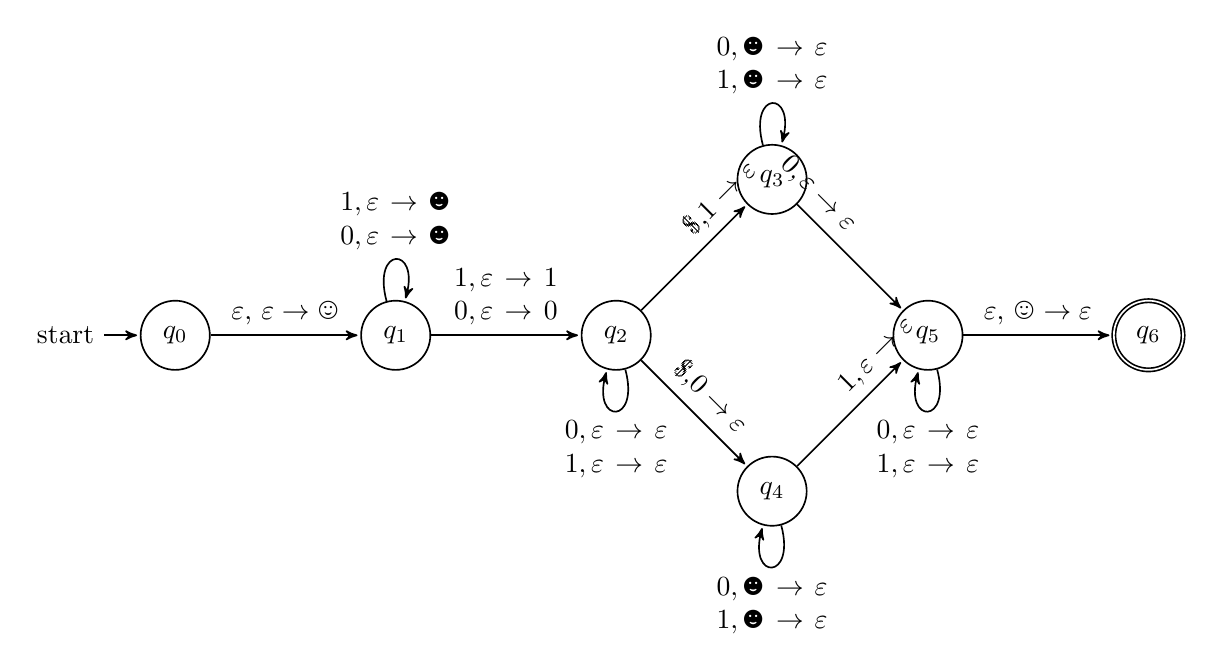
\begin{tikzpicture}[->,>=stealth',shorten >=1pt,auto,node distance=2.8cm,
                    semithick]
  \tikzstyle{every state}=[text=black]

  \node[initial,state] (A)                    {$q_0$};
  \node[state]         (B) [right of=A]       {$q_1$};
  \node[state]         (C) [right of=B]       {$q_2$};
  \node[state]         (D) [above right of=C] {$q_3$};
  \node[state]         (E) [below right of=C] {$q_4$};
  \node[state]         (F) [below right of=D] {$q_5$};
  \node[state,accepting]         (G) [right of=F] {$q_6$};

  \path (A) edge              node {$\varepsilon$, $\varepsilon \to \smiley{} $} (B)
        (B) edge [loop above] node[text width=2cm,align=center] 
            {$1, \varepsilon \to \blacksmiley{}$ \\
             $0, \varepsilon \to \blacksmiley{}$} (B)
            edge              node[text width=2cm,align=center] 
            {$1, \varepsilon \to 1$ \\
             $0, \varepsilon \to 0$} (C)
        (C) edge              node[pos=0.9, sloped] {\$,$1 \to \varepsilon $}  (D)
            edge              node[pos=0.5, sloped, above] {\$,$0 \to \varepsilon $} (E)
            edge [loop below] node [text width=2cm,align=center]
                                   {$0, \varepsilon \to \varepsilon $ \\
                                    $1, \varepsilon \to \varepsilon $} (C)
        (D) edge              node[pos=0.05,sloped] {$0, \varepsilon \to \varepsilon $} (F)
            edge [loop above] node [text width=2cm,align=center]
                                   {$0, \blacksmiley{} \to \varepsilon$ \\
                                    $1, \blacksmiley{} \to \varepsilon$} (D)
        (E) edge              node[pos=0.9, sloped] {$1, \varepsilon \to \varepsilon $} (F)
            edge [loop below] node [text width=2cm,align=center]
                                   {$0, \blacksmiley{} \to \varepsilon$ \\
                                    $1, \blacksmiley{} \to \varepsilon$} (E)
        (F) edge node {$\varepsilon$, $\smiley \to \varepsilon$} (G)
            edge [loop below] node[text width=2cm,align=center] 
                                   {$0, \varepsilon \to \varepsilon $ \\
                                    $1, \varepsilon \to \varepsilon $} (F)
        ;

\end{tikzpicture}

\textbf{b)}
For x and y to be different they have to be different in at least one place
\begin{align}
  \{0 \cup 1\}^a x_i \{0 \cup 1\}^b \{0 \cup 1\}^a y_i \{0 \cup 1\}^b \\
  \{0 \cup 1\}^a x_i \{0 \cup 1\}^a \{0 \cup 1\}^b y_i \{0 \cup 1\}^b 
\end{align}
Let $X = \{\{0 \cup 1\}^a x_i \{0 \cup 1\}^a \}$ and 
$Y = \{\{0 \cup 1\}^b y_i \{0 \cup 1\}^b\}$. We can construct a CFG \newline 
$G = (R,\{X,Y\}, \{0,1\}, S)$ for $L_2$ . With the following rules R: \\ \\
1) $S \to XY | YX$  \\
2) $X \to 0X0| 1X1 | 0X1 | 1X0 | 1$ \\
3) $Y \to 0X0| 1X1 | 0X1 | 1X0 | 0$
\end{problem}
\end{document}



 
% \begin{align}
% \end{align}
% \frac{}{}

